
\chapter{Materials and Methods} \label{sec:mm}

This chapter covers the images that were available to analyse, how they were processed, and which methods were applied to them. The details of the implementation of these methods are then discussed in Section \ref{sec:implementation}.

\section{Immune cells dataset}

\subsection{Setup}

The images that were used for the purpose of this research were provided by a researcher in Immunology at the University of Glasgow. The images were captured from multi-well plates with a commercial INCell Analyzer Machine\footnote{https://www.gelifesciences.com/en/us/shop/cell-imaging-and-analysis/high-content-analysis-systems/instruments/in-cell-analyzer-2500-hs-high-content-analysis-hca-imaging-system-p-04586}. As established in Section \ref{bg:immunesystem}, the type of immune cells we are studying are T-cells and dendritic cells (DCs). Each plate to be imaged in the INCell Analyzer Machine contains a grid of wells. Each well is assigned a label and an experimental condition. T-cells, dendritic cells, and compounds related to the experimental conditions are injected in the well. For distinction, the cells are loaded with fluorescent dyes: the T-cells are dyed with a green dye (FITC dye), and the dendritic cells are dyed with a red dye (TexasRed dye). After imaging, we obtain three field-of-view images per well:

\begin{itemize}
    \item a Brightfield image, which shows both T-cells and dendritic cells (Figure \ref{fig:fov_brightfield})
    \item an image showing only the T-cells, which has been captured thanks to the fluorescent green dye (Figure \ref{fig:fov_fitc})
    \item an image showing only the dendritic cells, which has been captured thanks to the fluorescent red dye (Figure \ref{fig:fov_tr}).
\end{itemize}

\begin{figure}[h]
    \centering
    \begin{subfigure}[h!]{0.3\textwidth}
        
\includegraphics[width=\textwidth]{dissertation/figures/example_Brightfield.png}
        \caption{Brightfield view}
        \label{fig:fov_brightfield}
    \end{subfigure}
    \begin{subfigure}[h!]{0.3\textwidth}
        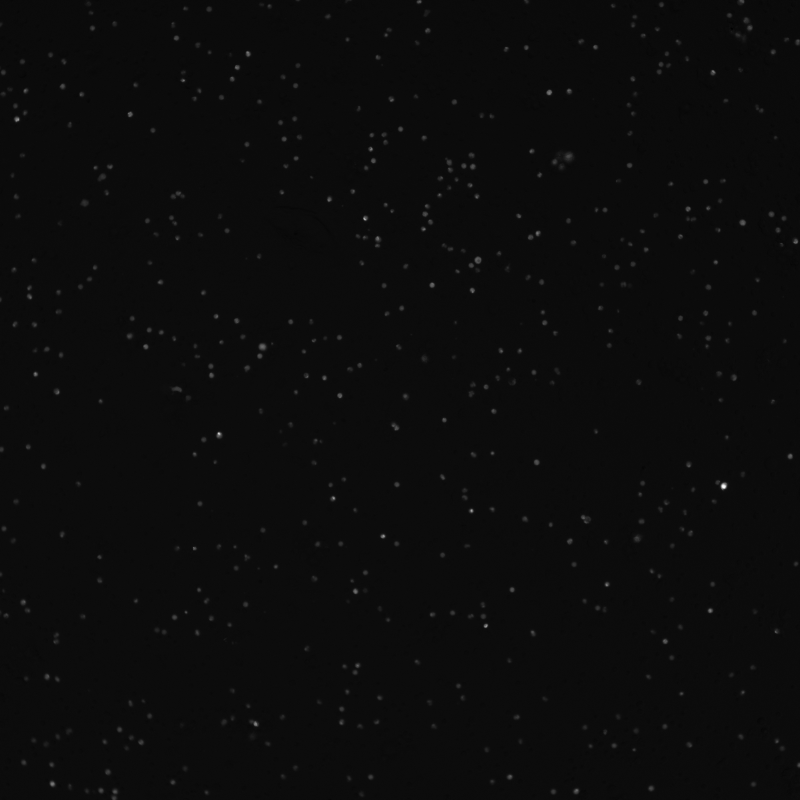
\includegraphics[width=\textwidth]{dissertation/figures/example_FITC.png}
        \caption{Green dye (T-cells) view}
        \label{fig:fov_fitc}
    \end{subfigure}
    \begin{subfigure}[h!]{0.3\textwidth}
        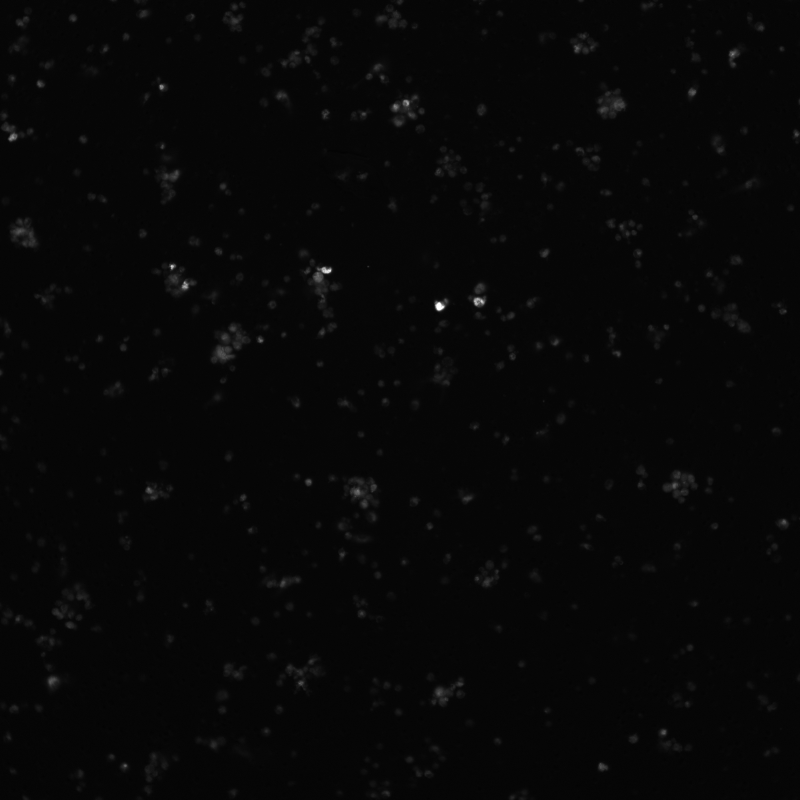
\includegraphics[width=\textwidth]{dissertation/figures/example_TexasRed.png}
        \caption{Red dye (DCs) view}
        \label{fig:fov_tr}
    \end{subfigure}
    \caption{Square patches from microscope field-of-view images, 33.3x zoom}
    \label{fig:fov}
\end{figure}

[change contrast of images -> tie in to dust point]

\subsection{Experimental conditions}

[need some explaining about labels and drugs here]

\subsection{Selecting images}

There was a large amount of images available from different well plates with different experimental conditions. However, each set of images represents about 8 GB of data on average. Moving images through disks or cloud filing system represented substantial time and was vulnerable to transfer errors. Hence, a limited number of plates were selection for training and evaluation to make sure their consistency could be validated. The plates chosen had to be picked keeping in mind the experimental conditions they represented. [make this clearer]

\begin{itemize}
    \item The ``DMSO" dataset: [TODO to be read over by Hannah] DMSO is a solvent that helps solubilise the drug compounds in a well as most compounds are not initially water soluble. The drug compounds being more soluble, they should then be able to have more of an impact.
    \item The ``balanced” dataset: this dataset contains an equal number of images in the three categories of stimulation: no drug stimulation, stimulation with OVA peptide, and stimulation with ConA. This is to fight issues of class imbalance when training the model.
    \item The simpler dataset, with two categories: this  dataset contains an equal number of images in two categories: no drug stimulation, and stimulation with OVA peptide. This was picked in the hope that if no results are obtained with 3 categories, a model might be able to perform better with two.
\end{itemize}

\subsection{Pre-processing}
The datasets obtained from this setup consisted of 2048x2048 16-bit images in TIFF format, captured by a 12-bit camera. As mentioned above, each ``image” consists in fact of a set of three views: the green fluorescent image (T-cells), the red fluorescent image (dendritic cells), and the Brightfield image. The Brightfield images show both cell types and can be used for diagnostic purposes when deciding on pre-processing methods, but were otherwise discarded and not used for further analysis.

%Fiji (ImageJ) was used to explore the images as the particular 12-bit format of the image in a TIFF file meant that standard image previewers reproduced the image as all black. Fiji also offered useful tools for testing image pre-processing methods, such as binary filters, thresholding, and background correction.
Each of the images sized about 8MB, and represented 4,194,304 pixels. Each plate had about 400 wells, which corresponds to 800 images when counting both the T-cell image and the DC image. This represented an issue of very high dimensions to deal with, and little images to feed into any kind of model.

Moreover, Figures \ref{fig:fov_fitc} and \ref{fig:fov_tr} shows that even to the naked eye, the smaller white dots could easily be confused for dust on the screen, and could be as confusing for a deep learning model trying to learn features from an image as they are for us. Furthermore, they remained of very high dimensions. A basic autoencoder with three 2x2 Pooling operations would yield around 500,000 pixel points, which is a very high number for a visualisation technique like t-SNE or UMAP.

\bigskip
\subsubsection{Sliding window}

\hfill\\
\hfill\\
To resolve this issue, the first idea was to make the images more palatable by a neural network by cropping a set square subsection of the image of smaller dimensions, e.g. 250x250. However, this would still leave an issue of having limited input to train a neural network. Instead, images were pre-processed by passing a sliding window over the image, creating patches of images per file. This quickly expanded the size of the dataset, making it as big as 58,000 samples in some cases. Smaller images also made more sense to the naked eye, hence the assumption was made that a trained neural network would perform better on this gridded dataset than on a full-image dataset.

[how many image patches per image?]

\bigskip
\subsubsection{Noise detection and normalisation}

\hfill\\
\hfill\\
[make sure to talk about things in logical order]

[coincidence of 0,255 range or not?]

From analysing the images, it was also found that some images contained a lot of pixels in the range of [0, 255] before normalisation. Moreover, these pixels seemed to be background noise as shown in Figure \ref{fig:bgnoise}. The immunology researcher providing the images confirmed that this noise was present in some images read from specific plates. Wells in early experiments were injected with additional cells as researchers thought this made the cells `happier' [ask Hannah how to best say this], however this was found to make no change. These cells were not dyed, but some of their details still came through the imaging system. Although this background was not always visible to the naked eye, we did not want those pixel values to confuse a neural network model. Hence, values below 255 in images were clipped to 255.

\begin{figure}[h!]
    \centering
    \begin{subfigure}[h!]{0.99\textwidth}
        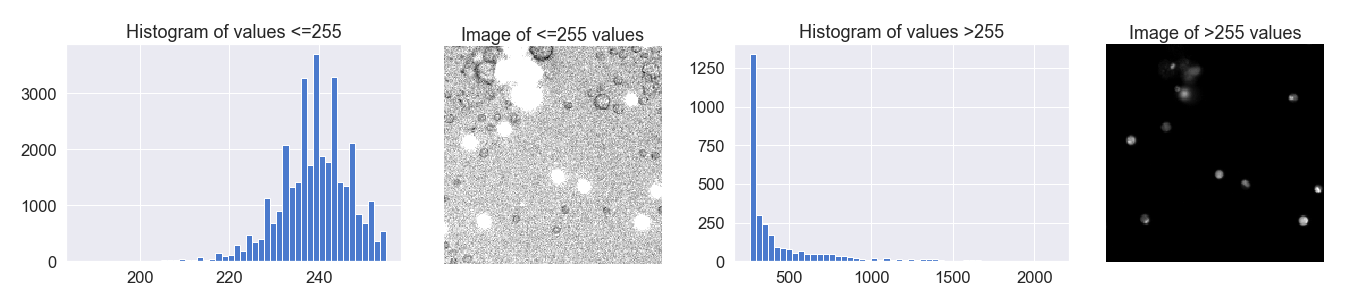
\includegraphics[width=\textwidth]{dissertation/figures/background_noise_true.png}
        \caption{Histogram and image analysis for a sub-image with noisy cells in the background}
        \label{fig:bgnoisetrue}
    \end{subfigure}

    \begin{subfigure}[h!]{0.99\textwidth}
        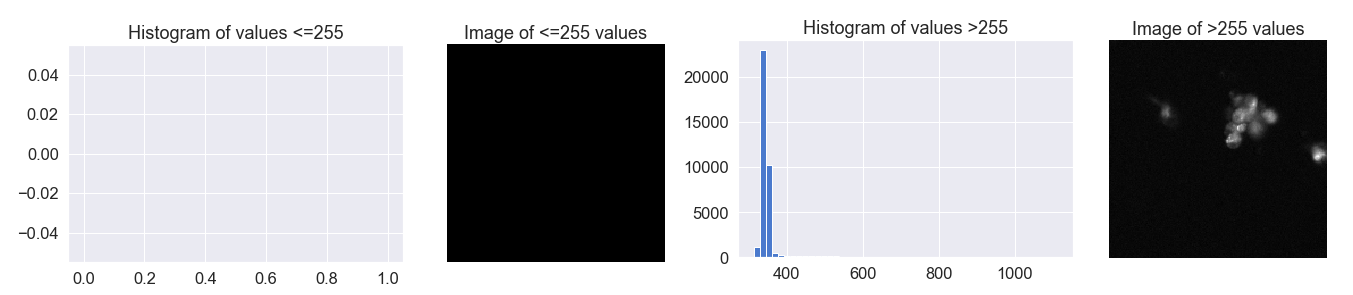
\includegraphics[width=\textwidth]{dissertation/figures/background_noise_false.png}
        \caption{Histogram and image analysis for a sub-image with no noisy cells in the background}
        \label{fig:bgnoisefalse}
    \end{subfigure}

    \caption{Histogram and image analysis for background noise detection}
    \label{fig:bgnoise}

\end{figure}

[label histogram images]

Each sub-image was then normalised with min-max normalisation (\autoref{equation:minmax}) to get a [0,1] range of pixel values. [why? -> CVMA]

\begin{equation}
    minmax(x) = \frac{x - min(x)}{max(x) - min(x)}
\label{equation:minmax}
\end{equation}

\bigskip
\subsubsection{Outlier detection}

\hfill\\
\hfill\\
\begin{figure}[h]
    \centering
    \begin{subfigure}[h!]{0.3\textwidth}
        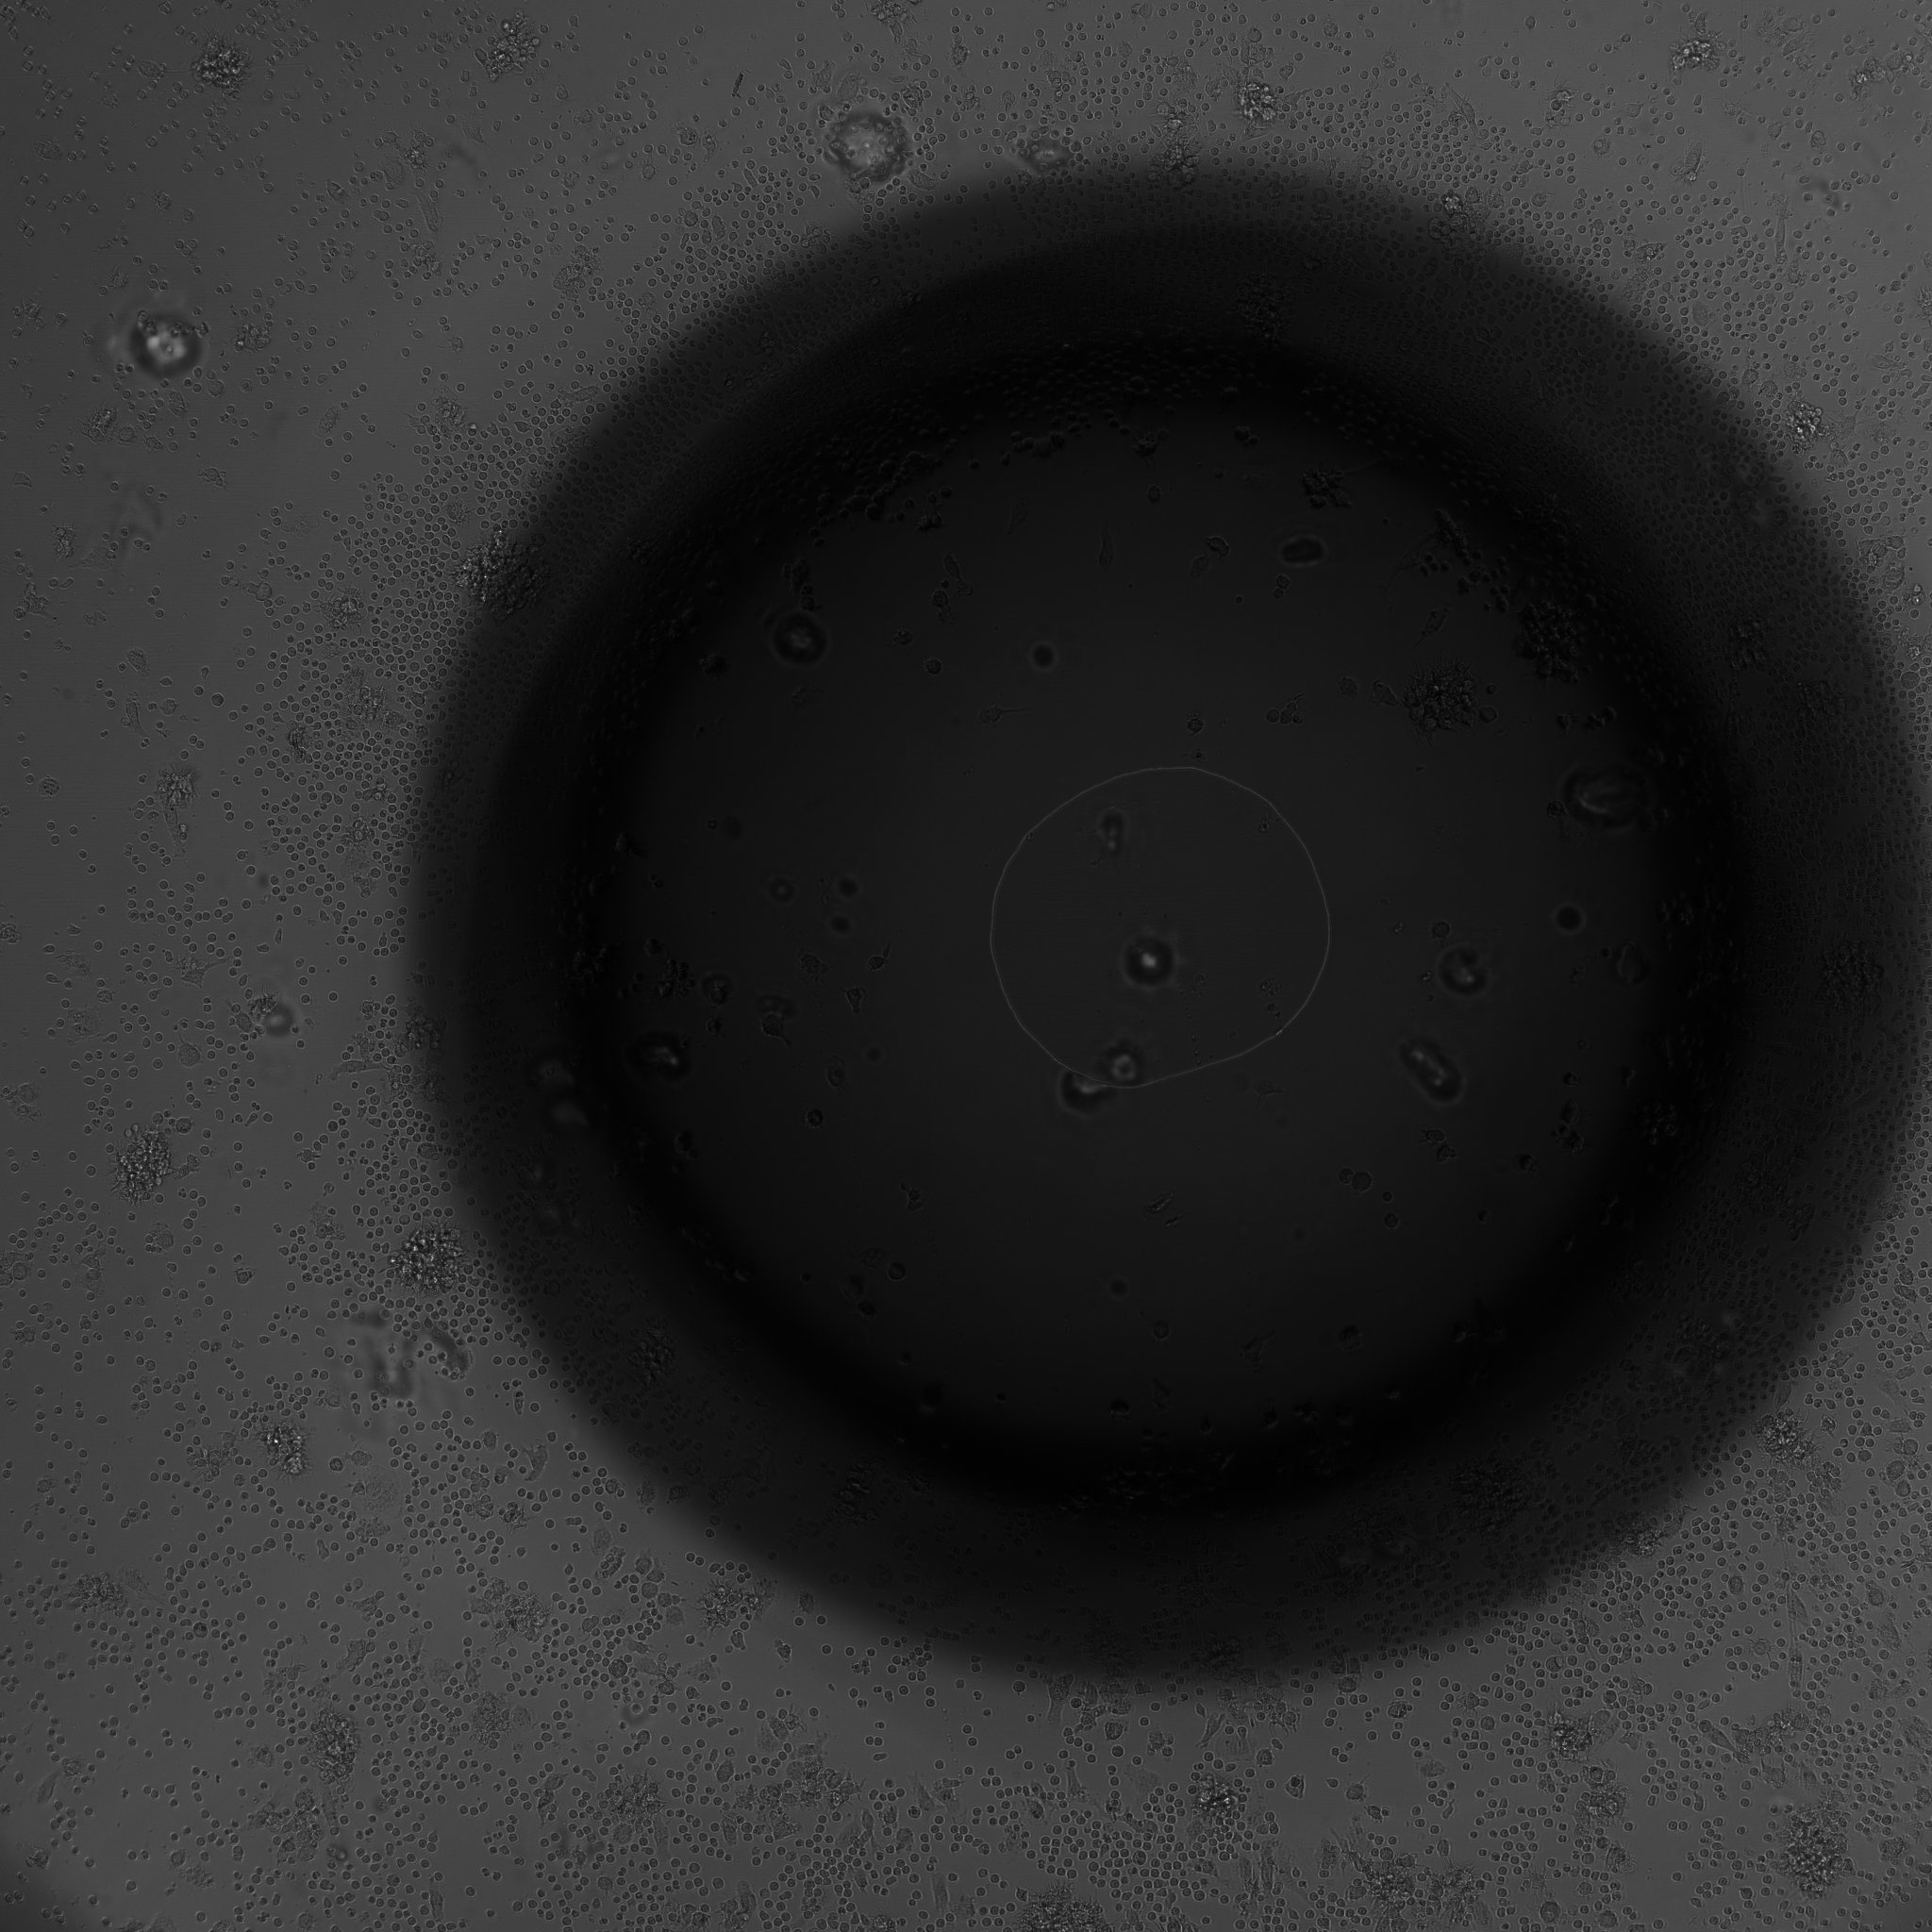
\includegraphics[width=\textwidth]{dissertation/figures/faulty_brightfield.jpg}
        \caption{Brightfield view}
    \end{subfigure}
    \begin{subfigure}[h!]{0.3\textwidth}
        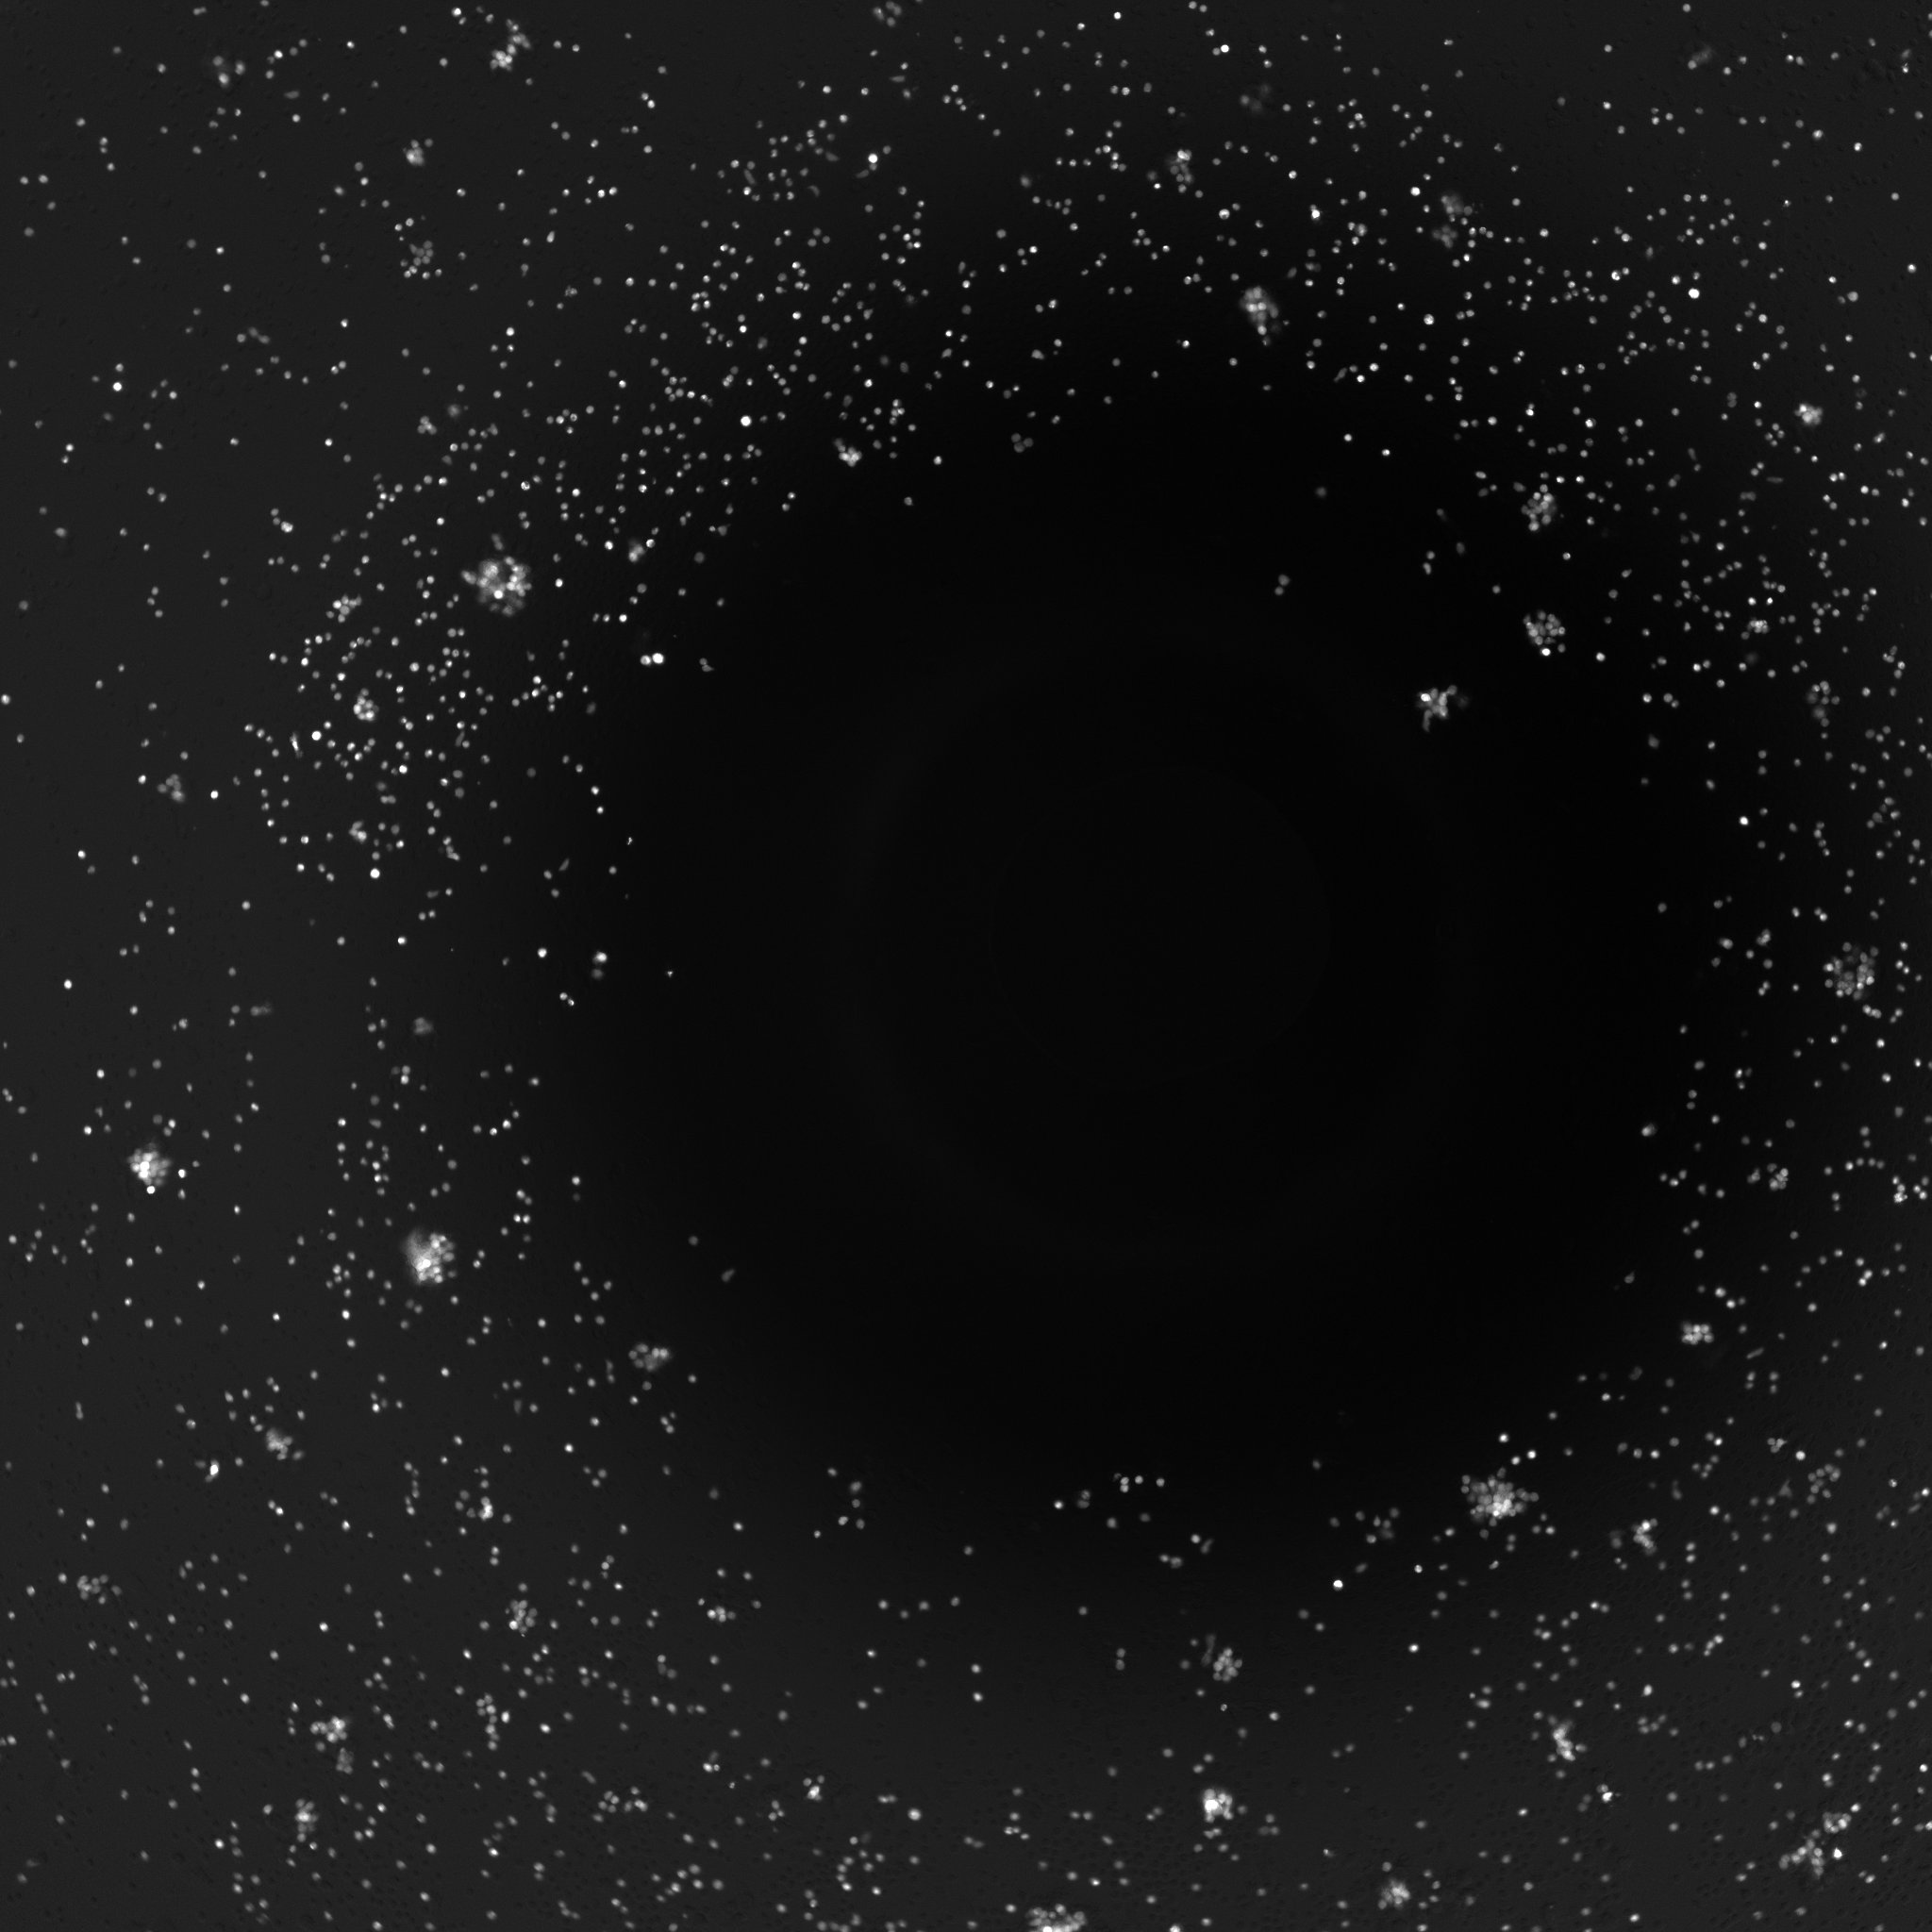
\includegraphics[width=\textwidth]{dissertation/figures/faulty_tcell.jpg}
        \caption{Green dye (T-cells) view}
        \label{subfig:tcell}
    \end{subfigure}
    \begin{subfigure}[h!]{0.3\textwidth}
        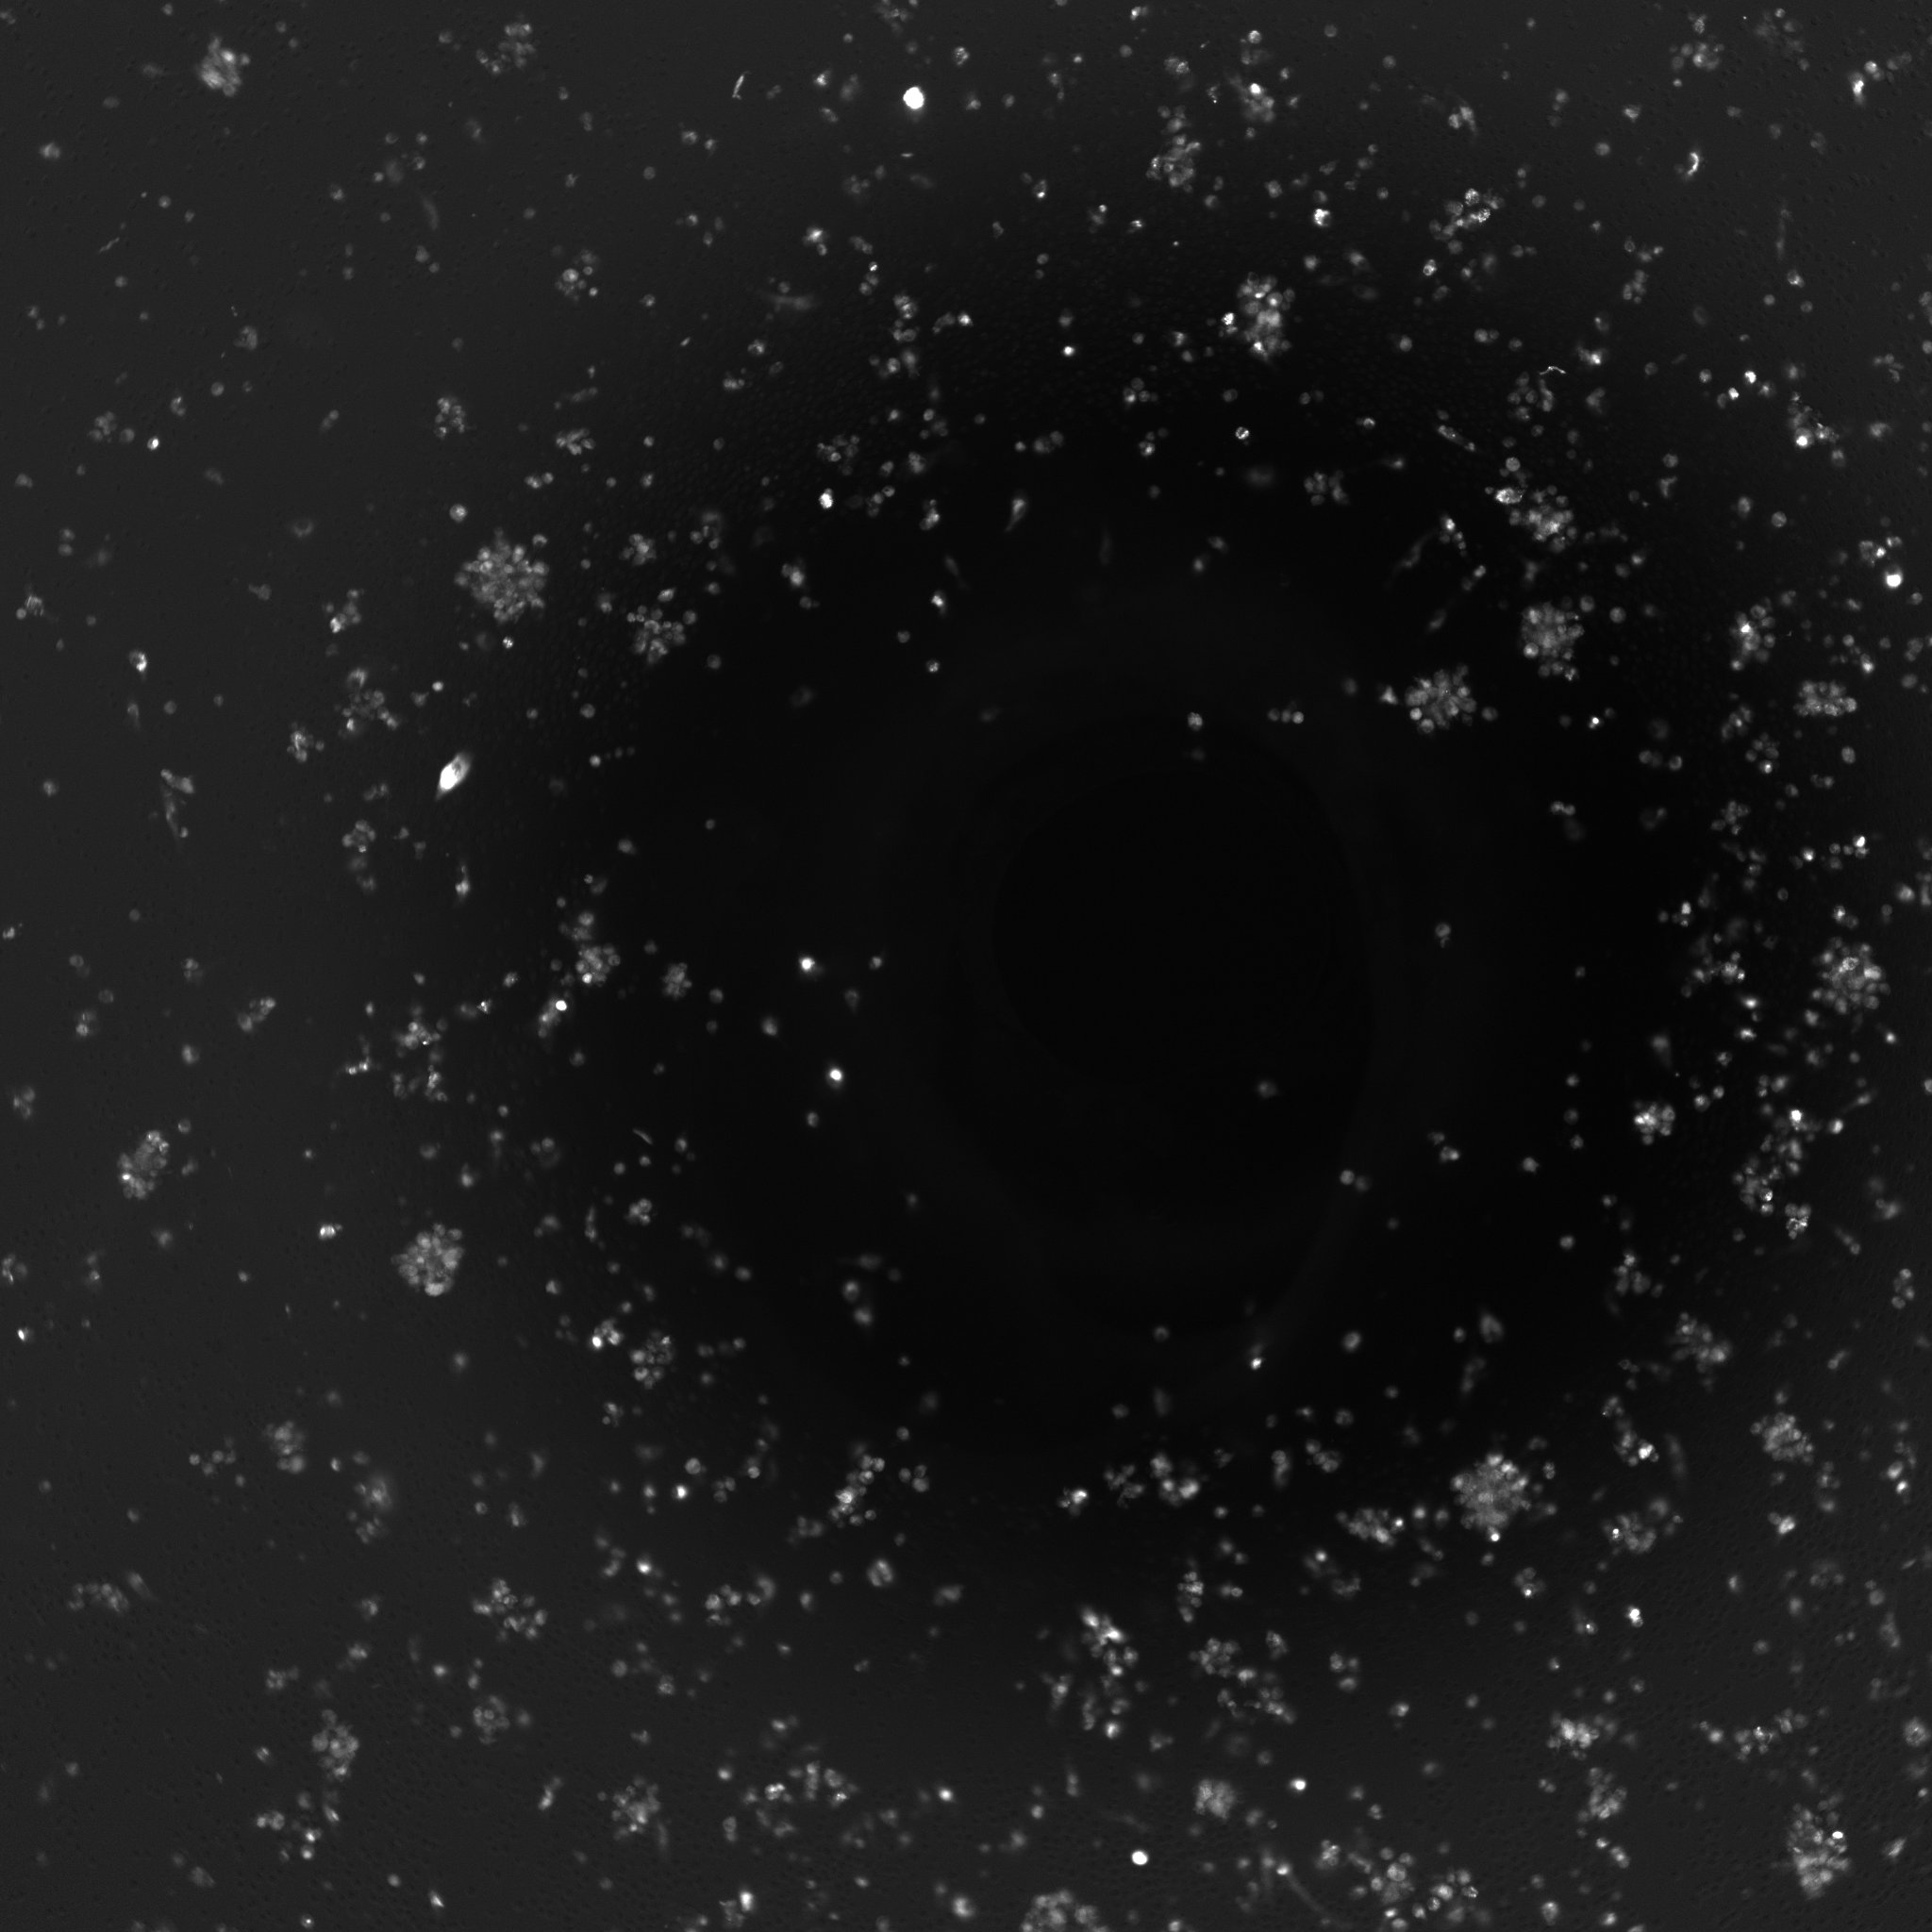
\includegraphics[width=\textwidth]{dissertation/figures/faulty_dcell.jpg}
        \caption{Red dye (DCs) view}
        \label{subfig:dc}
    \end{subfigure}
    \caption{Different views of an image which contains ``Faulty" patches. \protect\subref{subfig:tcell}, \protect\subref{subfig:dc} have been brightness-adjusted for visualisation.}
    \label{fig:noisyimage}
\end{figure}
As described above, the provided images sometimes contained some background noise. Furthermore, some images contained larger amounts of noise coming from defects in the well such as water droplets. This is illustrated in Figure \ref{fig:noisyimage}. Their pixel value distribution followed the [0, 255] range as described above but these values covered the whole sub-image and no cells of interest were present in those patches. Removing them entirely from the dataset made it more difficult to reason about whole images, as a full image is represented by 100 sub-images, and removing them would create inconsistencies in the amount of sub-images per image file. Instead of removing them, it was decided to keep them in to see if a neural network could make sense of them as a category. The noisy sub-images were labelled as ``Faulty".

\bigskip
\subsubsection{Labelling}

\hfill\\
\hfill\\
Each plate came with an Excel sheet giving information about the plate layout. Each image was given a letter and a name, and the Excel sheet gave information about drug stimulation, compound ID number, or compound concentration. These Excel sheets were not automatically parsable as types of drugs or location in the sheet might vary from one to the next, hence labelling had to be hardcoded and handchecked.

\subsection{Combining images to qualify interaction} \label{subsec:combining}

To summarise, we have established that for each well representing an experimental condition, we obtain two images of interest: an image of T-cells, and an image of dendritic cells. While these are obtained separately with the help of fluorescent dyes, they are still captured from the same well in which they are placed together. Hence, for us to gain any understanding of cell interaction from these images, we need to combine them one way or another.

We decided to combine each black-and-white T-cell and DC image in one RGB image. Computationally speaking, a RGB image corresponds to a multi-dimensional array of three arrays. Each of these arrays corresponds to a colour channel: red, green, and blue. The dendritic cell image has been obtained through fluorescent red dye screening, so the red channel of the image is set to this image. Similarly, the T-cell image has been obtained through fluorescent green dye screening, so the green channel of the image is set to this image. The blue channel of the RGB image is left blank. This RGB image allows us to visualise T-cells in green, DCs in red, and any close overlap between those cells will be in orange hues. Figure \ref{fig:combined} illustrates a sample of combined sub-images after this operation is completed.

This combination allows us to visualise areas of proximity in cells as well as areas of overlap. This visualisation is a means of qualifying interaction between the different types of immune cells.

\begin{figure}[h]
    \centering
    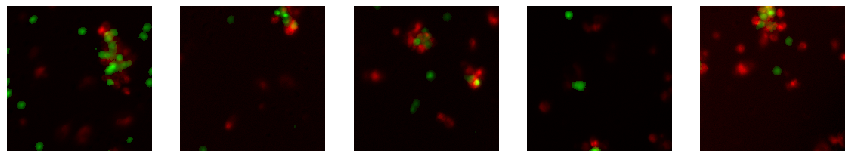
\includegraphics[width=\textwidth]{dissertation/figures/combined_cells.png}
    \caption{Random sample of five RGB images, where the red channel contains the dendritic cells and the green channel contains the T-cells.}
    \label{fig:combined}
\end{figure}

\section{Image segmentation}

Image segmentation refers to the process of separating out the parts of interest of an image into different `segments' or objects. In our context, applying image segmentation to our dataset had two purposes. The first was to use image segmentation as a method to separate the background from the cell objects for background correction. The second was to use it to obtain binary objects of the cells in order to compute numerical data about cells in the images.

\subsection{Background correction} \label{subsec:correction}

[explain why additional background correction step is necessary following the clipping you applied to the images with noisy backgrounds in section 3.1.4]

A common issue for microscope images obtained systematically through different screening systems is that of a noisy background [ref]. This can usually be corrected through different methods, such as flat field correction [ref]. Flat field correction removes image noise by using a ``neutral” background image without any additional objects (i.e. cells) as a reference image. However, the provided dataset did not come with a flat field image. As such, alternatives had to be explored.

All the images in the original, uncombined dataset are black and white, with the details of interest (the cells) in bright white spots. However, as discussed in Section \ref{subsec:preproc}, the image can contain noise coming from gray details in the image that the naked eye cannot see immediately, but that could influence how a model learns. Hence, we need a method that will separate out the cell pixels from the background. We can achieve this by obtaining a binary mask of the image, such that the white pixels of the binary image correspond to the cells, and the dark pixels correspond to the background. There are two ways of doing this which we will describe further in Section \ref{sec:implementation}: K-means segmentation, and thresholding.

Once a binary mask is obtained through these methods, we can remove the background of the original image by multiplying it with the mask, a procedure known as \textit{masking}. If the binary mask is satisfactory, the output of this image should only contain the cells, who will have kept their detail, while the background will have been blacked out.

\subsection{Quantifying interaction}

[make it clear this is not on combined images --> this is a different way of looking at interaction. However, the label will be attached to combined images.]

The process used in \autoref{subsec:combining} describes a way of visually qualifying interaction between immune cells. However, we are also interested in quantifying interaction and obtaining a numeric value for immune cell interaction observed in an image.

We can reuse the method described in subsection \ref{subsec:correction} for obtaining the mask of the cell objects. This mask can be used for further calculations. A common metric for evaluating image segmentation quality is Intersection over Union (IoU), also known as the Jaccard index [ref].

\begin{equation}
    IoU(X,Y) = \frac{X \& Y}{X | Y}
\end{equation}

In this case, we can use the IoU as a metric for area of overlap between two separate cell objects: the T-cell objects and the dendritic cell object obtained from the same image in the same experimental conditions. We can use the concept of overlap to quantify the level of interaction between cells. This number will then be used as a label input to a deep regression model. The aim will be to evaluate whether we can train a model to recognise a numeric value of interaction from an image.

\begin{figure}
    \centering
    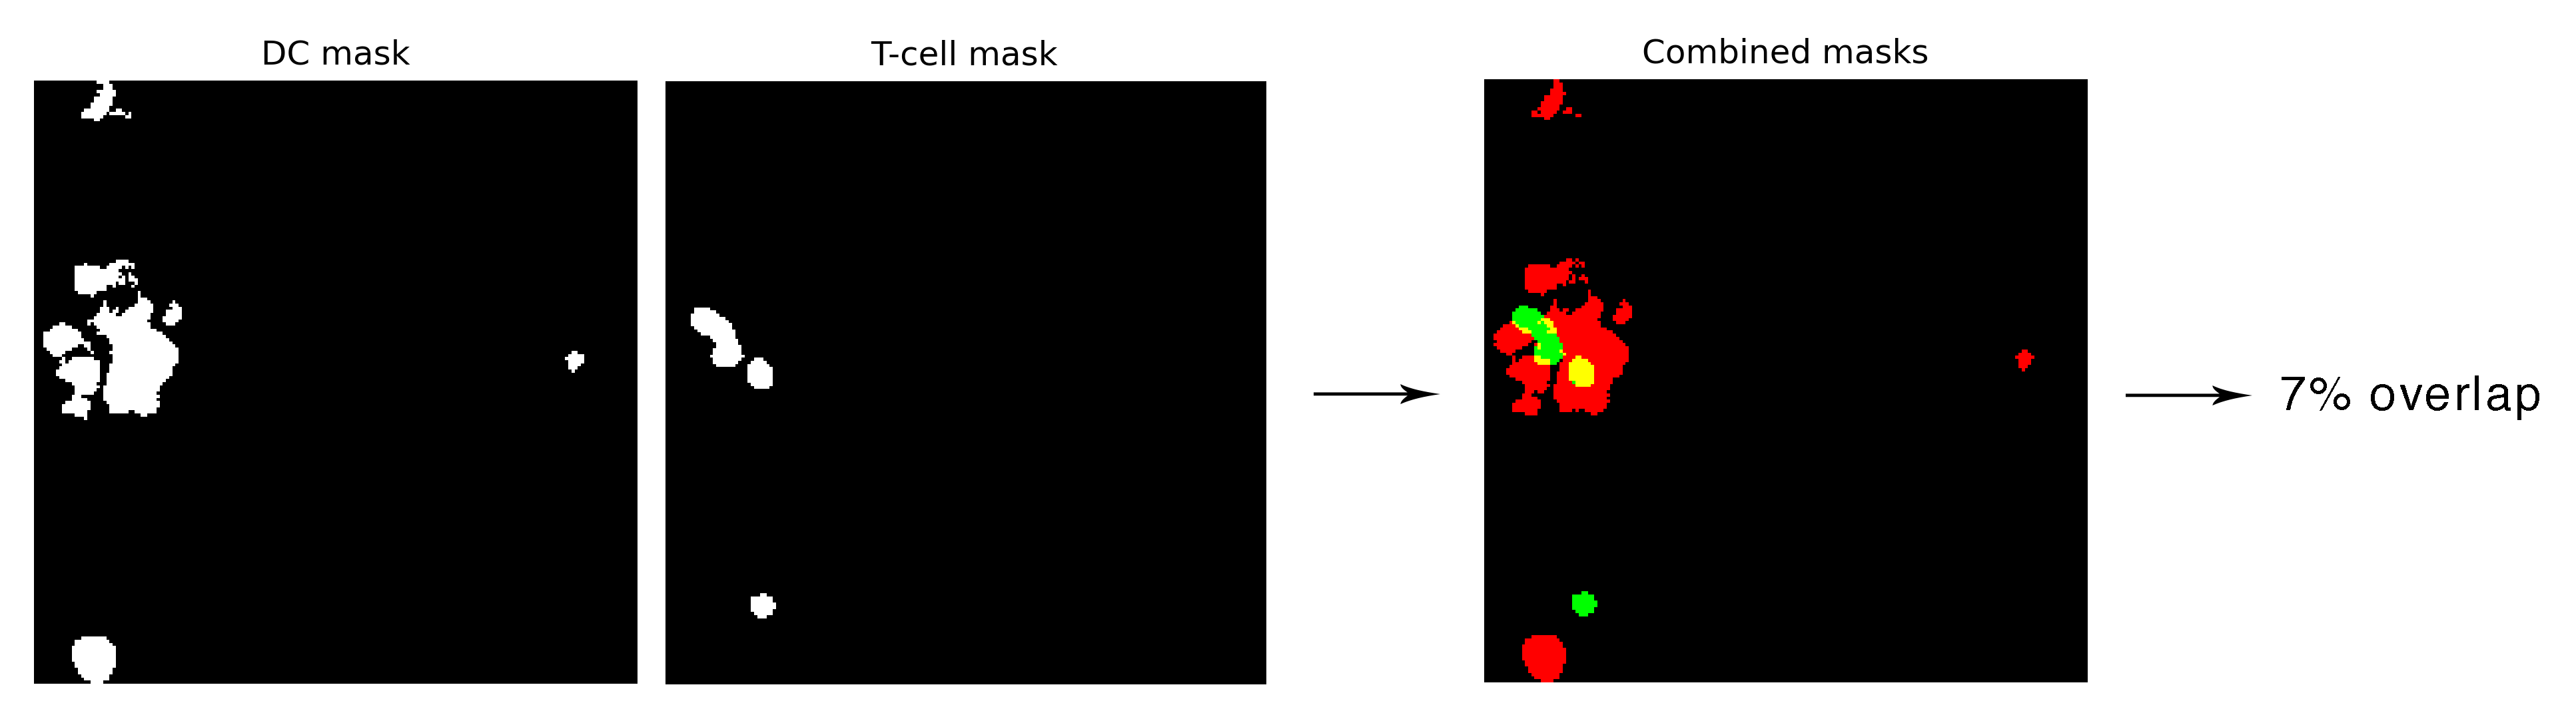
\includegraphics[width=0.8\textwidth]{dissertation/figures/mask_overlap_operation.png}
    \caption{Example of visual and numerical overlap between two sets of immune cells}
    \label{fig:mask_overlap}
\end{figure}

\section{Autoencoder}

As described in Section \ref{sec:research}, autoencoders are a particular type of neural network built with symmetrical layers around a bottleneck. The aim of an autoencoder is to map an input to itself as close as possible while reducing its dimensions. The hope is that if an image is reduced to a certain number of dimensions, and a neural network is able to reconstruct the original image very closely just based on that compressed representation, then that smaller code representing image is a good enough representation of the original input that can be fed into other models or algorithms.

[autoencoder figure here?]

The following two sections highlight the purposes of developing an autoencoder in the context of our research.

\subsection{Visualising high dimensional data}

The first use for our autoencoder is to reduce the dimensions of our image input, as the size of the data points will not only make it slow for data visualisation techniques to process, but also harder for them to distinguish any structure in the data. High dimensionality visualisation techniques such as t-sne and UMAP can help visualise if there is an inherent structure to the data. We want to use this as a tool for analysis of immune cells interactions. We want to evaluate whether or not a technique such as t-SNE or UMAP can cluster different images around similar experimental conditions. If such successful groupings were found, it would allow us to show that different drug compounds yield structurally similar cell interactions. The aim is to be able to qualify interaction from an image.

\subsection{Quantifying interaction in unseen images}

The second user of our autoencoder will be as a building block for a deep regression model. If our full autoencoder shows a satisfactory reconstruction performance, then we can use the encoder block of the model and extend it in a regression structure. This autoencoder-based regression model will take images and associated overlap values as input for training. We will then use the model to make predictions for overlap values on unseen images and assess whether or not it does so successfully. The aim is for our regression model to be able to quantify interaction from an image.
